\documentclass[a4paper, 11pt]{article}
\usepackage{template}

\title{Refactoring the Design of an Existing Project \\\large Software Design and Modeling, Università della Svizzera italiana}
\author{Luca Di Bello}
\date{\displaydate{today}}

\begin{document}
\maketitle

% Introduction: motivation, project selection, description of toolings that will be used
\section{Introduction and refactoring goals}
This assignment requires the use of the knowledge acquired during the course, in order to refactor an existing open-source project, aiming to improve its design. The behavior of the project should remain unchanged, as well as its input and output interfaces.

The refactoring should target at least 1000 lines of code, and the changes should be documented in a report, and pushed to a separate branch in the project's repository, allowing an easy comparison between the original and the new, improved version. To find valuable candidates for this assignment, the GitHub search feature was used, filtering the results by language, Java, and the number of stars, between 100 and 1000. The search results were sorted by last update date, in descending order in order to find active projects.

Additionally, each selected project size was analyzed with the web application \href{https://codetabs.com/count-loc/count-loc-online.html}{Count LOC}, in order to count the total lines of code (later referred as \emph{LOC}) that would be affected by the refactor (considering only source code, excluding tests or other utilities).

\subsection{Project selection}

As cited before, in order to accomplish the personal objective set at the beginning of this assignment, the search targeted project with a high number of stars, between 100 and 1000, and written in Java language in order to leverage the knowledge acquired during the course. The search results were sorted by the last update date, in descending order, to find active projects. After an in-depth analysis of results, these are the possible candidates selected for further investigation:

\begin{itemize}
	\item \href{https://github.com/flanglet/kanzi}{fanglet/kanzi}: Kanzi is a modern, modular and efficient lossless data compressor implemented entirely in java. It uses state-of-the art entropy coders and multi-threading in order to efficiently utilize multi-core CPUs. The design of the library is modular, allowing to select at runtime the best entropy coder for the data to compress. The project has 109 stars, 18 forks, no open issues, and approximately 20,000 LOC. Kanzi was initially selected for this assignment, but later discarded due to its size.
	\item \href{https://github.com/jinput/jinput}{jinput/jinput}: JInput is a Java library designed for accessing input devices such as game controllers, joysticks, and other peripherals. It provides a platform-independent API to facilitate the integration of various input devices into Java applications. The project has 150 stars, 79 forks, 29 open issues, and 10,000 lines of code (considering only core functionality, excluding tests). JInput was initially selected for this assignment, but unfortunately, after inspecting the codebase it was discarded as the project presented too many platform-specific implementations spanning multiple modules and a complete lack of documentation and tests. This would make the refactoring process too complex and time-consuming.
	\item \href{https://github.com/byronka/minum}{byronka/minum}: Minum is a minimalistic web framework written in Java, built from scratch using few dependencies. The project provides essential components for web application development, including a web server and an in-memory database with disk persistence. This project was particularly interesting as it emphasizes simplicity and minimalism, which is a good starting point for refactoring as most of the code is written from scratch without complex dependencies. Minum has 611 stars, 38 forks, no open issues, and approximately 5'500 LOC (excluding tests and comments). After a thorough analysis, this project was selected for refactoring as it presents a clear and concise codebase divided into several packages, which will allow for a more focused refactor. Furthermore, it presents a complete JavaDoc documentation, which will be useful to understand the project's design.
\end{itemize}

\noindent \textit{Note}: The data presented above was collected on the \displaydate{collectiondate}, and may have changed since then. Check the project's repository for the most recent information.

\subsection{High-level overview of the project structure}
\label{sec:project_structure}

The project presents a single \textit{Maven} module which contains the core functionality of the framework. The module contains 10 packages, each with a specific purpose. The following list provides a high-level overview of the purpose of each package:

\vspace{1em}
\noindent
\begin{minipage}{0.5\textwidth}
	\begin{itemize}
		\item \texttt{database}: In-memory database with disk persistence.
		\item \texttt{htmlparsing}: HTML parsing utilities.
		\item \texttt{logging}: Logging utilities.
		\item \texttt{queue}: Queue of tasks to be executed asynchronously.
		\item \texttt{security}: \href{https://github.com/fail2ban/fail2ban}{Fail2Ban}-like security mechanism and threat detection via log analysis.
	\end{itemize}
\end{minipage}
\begin{minipage}{0.5\textwidth}
	\begin{itemize}
		\item \texttt{state}: Singleton context to store global state.
		\item \texttt{templating}: Template engine to inject dynamic content into HTML pages.
		\item \texttt{testing}: Minimalistic testing framework for unit and integration tests.
		\item \texttt{utils}: General utilities.
		\item \texttt{web}: Web server and request handling.
	\end{itemize}
\end{minipage}
\vspace{1em}

\noindent From a first glance, the project seems well-structured, with clear separation of concerns between packages. As cited before, the codebase is well-documented, with JavaDoc comments present in most classes and methods, providing a good starting point to understand the project's design. In \autoref{sec:project_health_analysis}, the project design will be analyzed in more detail, focusing on the use of design patterns and potential code smells.

\subsection{Additional tools and resources}
\label{sec:additional_tools}

In order to perform a comprehensive refactor of the project, the \href{https://www.sonarsource.com/}{SonarQube} static code analysis tool will be used to identify potential code smells, bugs, and vulnerabilities, while also providing insights into the overall code quality. Additionally, in order to have a more in-depth understanding of the current design of the project, the \href{https://users.encs.concordia.ca/~nikolaos/pattern_detection.html}{Pattern4j} tool will be used to detect the use of design patterns in the codebase, an essential aspect of the refactoring process.

The results of both tools provide valuable information to guide the refactor, highlighting areas of improvement and potential refactoring opportunities, and, by combining both outputs, will be possible to have a more comprehensive view of the project's design and code quality.

\subsection{Building the project}

The Minum project uses Maven as the build system, and in order to simplify the configuration process, the creator of the library created a Maven Wrapper script (named \texttt{mvnw}) which is a self-container script that allows to automatically download the necessary Maven version to build the project. This ensures that the build process is reproducible across different environments. This script is located in the root of the project, and can be used to build the project by running the following command:

\begin{center}
	\begin{minipage}{0.5\textwidth}
		\begin{lstlisting}[language=bash, caption={Building the project using the Maven Wrapper script}]
    ./mvnw clean install
  \end{lstlisting}
	\end{minipage}
\end{center}

\noindent \textit{Note}: If the current environment already has Maven installed, the project can be built using the \texttt{mvn} command instead of the wrapper script.
\vspace{1em}

\noindent The build artifacts can be found in the \texttt{target} directory. The bytecode generated by the build process will be used by the \textit{Pattern4j} tool to analyze the project's design (refer to \autoref{sec:additional_tools}).


% Project health analysis: detected code smells, bugs, vulnerabilities, and design patterns
\section{Project health analysis}
\label{sec:project_health_analysis}
The project will be analyzed using both \href{https://www.sonarsource.com/}{SonarQube} and \textit{Pattern4j} tools. In the following section, the results of the analysis will be presented, highlighting potential code smells, bugs, vulnerabilities, and design patterns detected in the project.

As the configuration and usage of both tools is out of the scope of this report, the following sections will focus on the results of the analysis, providing insights into the current state of the project, and guiding the refactoring process. Refer to the respective documentation for more information on how to configure and use both tools.

\subsection{SonarQube analysis}

After running the SonarQube analysis on the entire Minium codebase (including tests in order to get the test coverage metric), were detected a total of 588 code smells, 26 security hotspots and 34 possible bugs. In the following paragraphs the results will be briefly analyzed in order to plan the refactoring process.

\paragraph*{Code smells} Out of the 588 code smells detected in the project, 109 of them are categorized as critical, 74 as major, and 405 as minor. \autoref{tab:sonarqube_severity_summary} provides a summary of the found code smells, categorized by severity.

\begin{table}[H]
	\centering
	\caption{SonarQube Severity Issues Summary}
	\label{tab:sonarqube_severity_summary}
	\begin{tabular}{|c|p{14cm}|}
		\hline
		\textbf{Severity Type} & \textbf{Issues}                                                \\ \hline
		\textbf{Critical}      &
		\begin{tabular}[t]{@{}l@{}}
			design (90), suspicious (10), brain-overload (6) convention (1), multi-threading (1), \\
			pitfall (1)                                                                           \\
		\end{tabular}   \\ \hline
		\textbf{Major}         &
		\begin{tabular}[t]{@{}l@{}}
			cert (40), html5 (20), obsolete (19) bad-practice (17), owasp-a3 (17), cwe (16), \\
			error-handling (15), pitfall (8), suspicious (7) accessibility (5), unused (4),  \\
			wcag2-a (4) confusing (2), design (2), brain-overload (1)                        \\
		\end{tabular}        \\ \hline
		\textbf{Minor}         &
		\begin{tabular}[t]{@{}l@{}}
			convention (374), cwe (7), java8 (5), brain-overload (4), pitfall (4), performance (2), \\
			regex (2), unused (2), bad-practice (1), clumsy (1), suspicious (1)                     \\
		\end{tabular} \\ \hline
	\end{tabular}
\end{table}

\noindent As shown in Table \ref{tab:sonarqube_severity_summary}, the most common code smells in the project are related to Java conventions, design issues, CERT secure coding standards, and the use of HTML5 in comments.

The refactoring of this project will focus on design, convention and brain-overload, as they are more related to the design and organization of the code, and can have a significant impact on the maintainability and readability of the project.

\paragraph*{Security hotspots and bugs} As cited before, the SonarQube scanner detected several bugs and security hotspots in the project. The security hotsposts are related to possible \textit{Denial of Service} attacks leveraging Regular Expressions backtracking and log injection vulnerabilities.

The log injection issue on the other hand is related to the use of the \texttt{Logger} class without proper sanitization of the logger name, which can lead to log injection attacks.

Both security hostspots will be addressed in the refactoring process in order to enhance the security of the project.

\subsection{Pattern4j analysis}

Unfortunately, the pattern4j tool was not able to analyze the entire project codebase due to the use of Java 21 features in the project. By running the tool using the custom \texttt{run-pattern4j-headless.sh} script, the following error was raised:

\begin{verbatim}
Exception in thread "main" java.lang.IllegalArgumentException: Unsupported class file major version 65
\end{verbatim}

\noindent For this reason, the design pattern usage anaylsis will be skipped. Fortunately, this step is not crucial for the refactoring of the project as it would have only provided additional insights into the design of the project rather than pinpointing specific issues.

\subsection{Main Issues and Refactoring Plan}

In the following sections, the most important code smells and design issues will be presented, along with a refactoring plan to address them. This allows the reader to understand the current state of the project and the steps that will be taken to improve it.

\subsubsection{Codebase Structure}

As cited in \autoref{sec:project_structure}, the project codebase is divided into 10 packages, each with a specific purpose. The overall structure of the codebase is showcase a very thorough organization, with each package containing a set of classes and interfaces related to a specific aspect of the library. However, by inspecting in more detail the structure of single packages four main issues were identified:

\begin{enumerate}
	\item The framework defines many custom exceptions in order to handle specific errors. These exceptions are scattered across the codebase and are not properly organized. This makes it difficult to understand the error handling mechanism of the library.
	\item Especially the \texttt{util} package, contains many self-contained classes that perform specific tasks. These classes are properly documented but are not properly organized hierarchically. Also, most of these utility classes have multiple responsabilities (i.e, function to convert a string to bytes, and also methods related to authentication).
	\item Model classes and interfaces are not properly organized in the \texttt{model} package. Each package contains a set of classes and interfaces related to a specific aspect of the library. This makes packages unnecessarily large and difficult to navigate. A better approach would be to use the a layered-architecture (model, service, repository) to organize the codebase.
	\item There are test classes inside the \texttt{main} package, which should be moved to the \texttt{test} package. Some of them (i.e., \texttt{FullSystemTests}) have empty methods, without comments or assertions, which should be removed.
\end{enumerate}

\subsubsection{Java Conventions, Duplicated Code and General Design Issues}

Especially inside test classes, the code is not properly organized, presenting multiple problems such as duplicated code, misuse of Java naming conventions and name shadowing. As test classes are not part of the final library, these issues will not be addressed in the refactoring process.

On the other hand, the main codebase presents problems that must be addressed. The following list summarizes the main issues found in the project:

\begin{itemize}
	\item Class/interface naming issues: there are classes which do not follow neither the Java naming conventions nor the project naming conventions. For example: \texttt{TheBrig}/\texttt{ITheBrig}, \texttt{SetrfSws}, \texttt{MyThread}.
	\item Reuse of fixed values: there are fixed values used in multiple classes, which should be extracted into constants. For example, inside the \texttt{TheRegister} class,
	\item Even if there is a \texttt{Logger} class, there are many \texttt{System.err.println} statements in the codebase, which should be replaced by proper logging.
\end{itemize}



\subsubsection{Class-specific issues and Possible Design Patterns usage}

\paragraph*{\texttt{Response} class} Inside the \textit{com.renomad.minum.web.Response} class there are different methods to build different kinds of response. This could be a good candiate in order to use the \textit{Factory Method} along with the \textit{Chain of Responsability} pattern, in order to streamline the response building process and make it more modular.

\paragraph*{\texttt{WebFramework} class} The \texttt{com.renomad.minum.web.WebFramework} class is the main entry point of the library, and is responsible for handling the HTTP requests and responses after the socket connection. This class is too large (around 845 LOC), and contains many methods that are not directly related to the main responsability of the class.



\section{Refactoring process}
\label{sec:refactoring}
In the following subsections, each step of the planned refactoring presented in \autoref{sec:refactoring_plan} will be detailed, providing insights into the previous state of the project, and the results achieved though the refactoring.

\subsection{\texttt{logging} package refactoring}

Within this package, the \texttt{Logger} class supports four logging levels: \texttt{DEBUG}, \texttt{TRACE}, \texttt{AUDIT}, and \texttt{ASYNC\_ERROR}, which are defined in the \texttt{LoggingLevel} \texttt{Enum}. To enhance flexibility, the library maintains the current state of these logging levels in a \texttt{HashMap}, where each entry is represented as a record \texttt{<LoggingLevel, Boolean>}. In this mapping, the key corresponds to a specific logging level as an \texttt{Enum}, and the value is a boolean indicating whether that level is enabled.

The library also includes a test example that demonstrates how to extend the built-in logger by defining a \texttt{DescendantLogger} class, which extends the \texttt{Logging} class in order to support a new set of logging levels encoded as the \texttt{CustomLoggingLevel} \texttt{Enum}. However, since there is no inheritance between \texttt{CustomLoggingLevel} and \texttt{LoggingLevel}, the library requires creating a separate \texttt{HashMap} to store the new logging levels. This approach results in code duplication, as the \texttt{DescendantLogger} class must reimplement all methods for managing logging levels, such as enabling/disabling levels, checking if a level is enabled, and logging messages at specific levels. This violates the DRY (\href{https://en.wikipedia.org/wiki/Don%27\_repeat\_yourself}{Don't Repeat Yourself}) principle and increases the overall complexity of the codebase.

To address these design issues and create a more flexible and maintainable solution, a new abstract class, \texttt{BaseLogger}, was created. This class encapsulates the necessary data structures to manage any set of logging levels defined as \texttt{Enum} objects implementing the \texttt{ILoggingLevel} interface. This allows to store logging levels in a single \texttt{HashMap} regardless of their type, thus reducing code duplication and improving maintainability. Furthermore, a new generic interface, \texttt{ILogger<ILoggingLevel>}, was introduced. This interface includes a method, \texttt{log(String, ILoggingLevel)}, which is implemented by the \texttt{BaseLogger} class. This improved design is illustrated in \autoref{fig:refactored_logging}.

% Logging package original
\begin{minipage}{0.4\linewidth}
	\begin{figure}[H]
		\begin{center}
			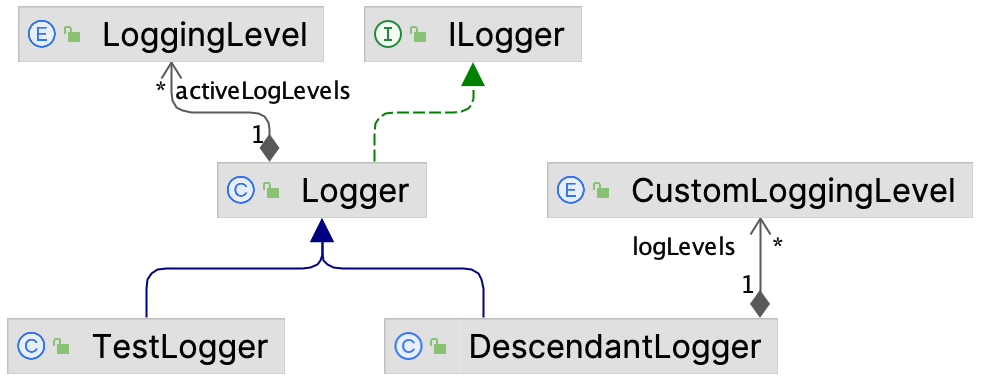
\includegraphics[width=0.95\textwidth]{figures/logging_package/original.png}
			\caption{Original \texttt{logging} package}
			\label{fig:original_logging}
		\end{center}
	\end{figure}
\end{minipage}
\begin{minipage}{0.6\linewidth}
	\begin{figure}[H]
		\begin{center}
			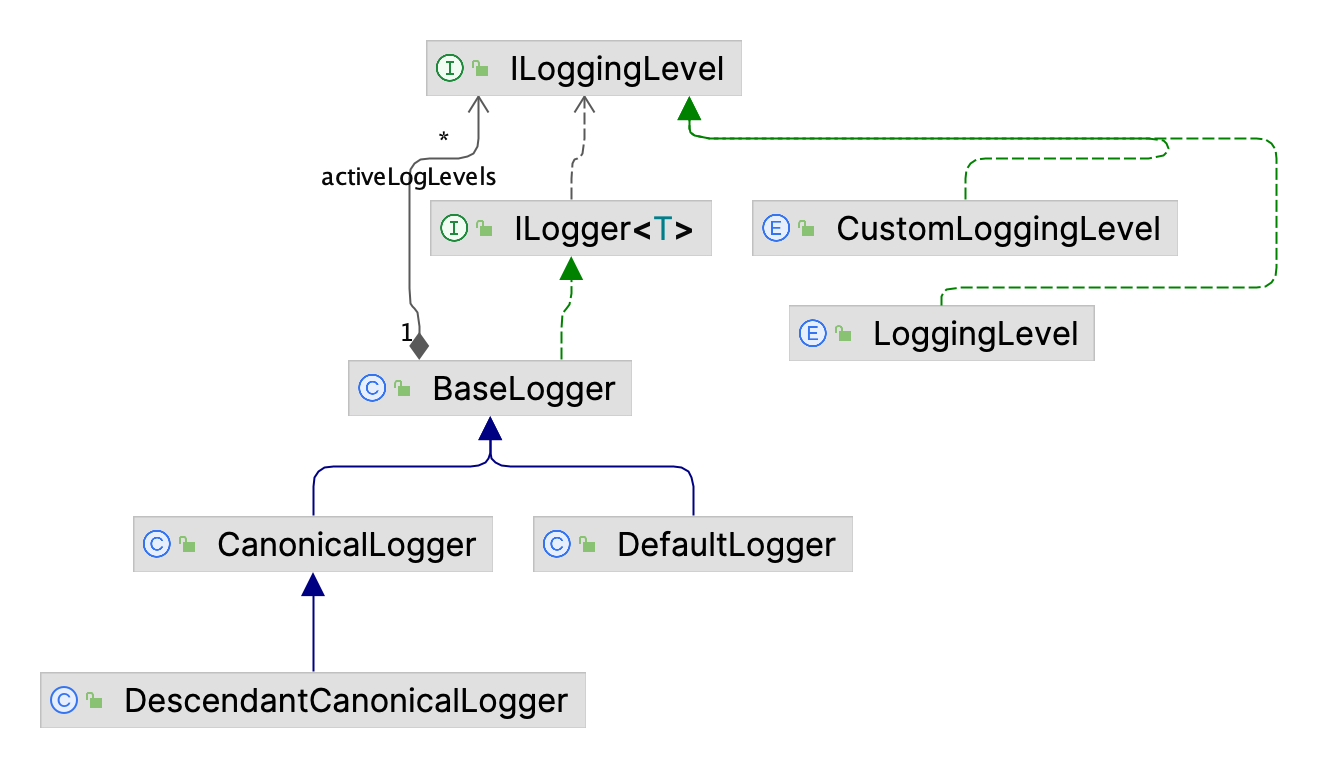
\includegraphics[width=0.95\textwidth]{figures/logging_package/refactored.png}
			\caption{Refactored \texttt{logging} package}
			\label{fig:refactored_logging}
		\end{center}
	\end{figure}
\end{minipage}

\noindent By adopting this approach, developers can define custom logger classes by simply creating new logging levels in an \texttt{Enum} that extends the \texttt{ILoggingLevel} interface. This eliminates the need to reimplement methods for managing logging levels or duplicating \texttt{HashMap} logic. As a result, the new architecture simplifies development and ensures adherence to the DRY principle.

As the \texttt{Logger} class was extensively used inside the core library, the refactoring process required updating all references to the \texttt{Logger} class to use the new \texttt{CanonicalLogger} class, which defines the default logging levels present in the original implementation to ensure backward compatibility. This was a long and tedious process, but it was necessary to ensure that the library maintained the same behavior as before.

Furthermore, also the proposed example of extension of the \texttt{Logger} class was refactored. Now, the \texttt{CanonicalLogger} class can be extended to support custom logging levels by simply defining a new \texttt{Enum} that implements the \texttt{ILoggingLevel} interface. This architecture allows an easy extension and customization of logging levels, as it is only necessary to define a new \texttt{Enum} that extends the \texttt{ILoggingLevel} interface and implement the required methods.

In the new test case, \texttt{DescendantCanonicalLogger} (previously \texttt{DescendantLogger}) implements an additional logging level \texttt{REQUEST} while still supporting the logging levels of the \texttt{CanonicalLogger} class. This demonstrates how the new architecture simplifies the process of extending the \texttt{Logger} class to support custom logging levels.

\subsection{Exception classes refactoring}

All exception classes are now in a single \texttt{exception} package in order to tidy up the codebase. The original design had exception classes scattered throughout the codebase, which made it difficult to locate and manage them.

\subsection{\texttt{queue} package refactoring}

The library defines a class \texttt{ActionQueue} that represents a queue of actions to be executed asynchronously by a thread. It receives a list of actions and executes them in the order they were added. For the development of the library, it was necessary to create a new class, \texttt{LoggingActionQueue}, which executes actions in a slight different way than \texttt{ActionQueue}. With the current architecture, \texttt{LoggingActionQueue} is almost an exact copy of \texttt{ActionQueue}. Refer to \autoref{fig:original_queue} for UML diagram of the original design.

To solve this issue, a new abstract class, \texttt{BaseActionQueue}, was created. This class encapsulates the common logic between \texttt{ActionQueue} and \texttt{LoggingActionQueue}, allowing to reduce code duplication and improve maintainability. After further analysis, was possible to remove completely the \texttt{LoggingActionQueue} class, as it was no longer necessary. The new design is illustrated in \autoref{fig:refactored_queue}.

% Logging package original
\begin{minipage}{0.5\linewidth}
	\begin{figure}[H]
		\begin{center}
			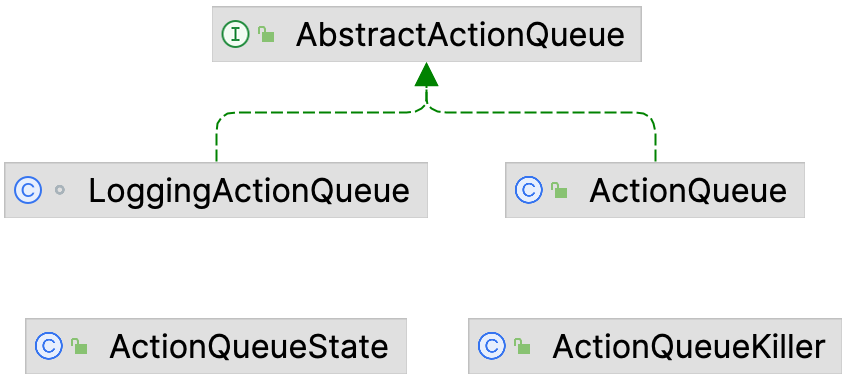
\includegraphics[width=0.95\textwidth]{figures/queue_package/original.png}
			\caption{Original \texttt{queue} package}
			\label{fig:original_queue}
		\end{center}
	\end{figure}
\end{minipage}
\begin{minipage}{0.5\linewidth}
	\begin{figure}[H]
		\begin{center}
			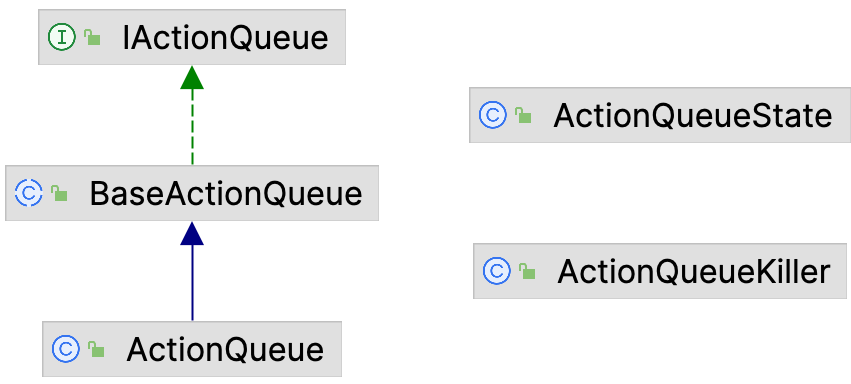
\includegraphics[width=0.95\textwidth]{figures/queue_package/refactored.png}
			\caption{Refactored \texttt{queue} package}
			\label{fig:refactored_queue}
		\end{center}
	\end{figure}
\end{minipage}



\section{Results and discussion}
\label{sec:results_conclusions}



\end{document}
